%  LaTeX support: latex@mdpi.com
%  For support, please attach all files needed for compiling as well as the log file, and specify your operating system, LaTeX version, and LaTeX editor.

%=================================================================
% pandoc conditionals added to preserve backwards compatibility with previous versions of rticles

\documentclass[data,article,submit,moreauthors,pdftex]{Definitions/mdpi}


%% Some pieces required from the pandoc template
\setlist[itemize]{leftmargin=*,labelsep=5.8mm}
\setlist[enumerate]{leftmargin=*,labelsep=4.9mm}


%--------------------
% Class Options:
%--------------------

%---------
% article
%---------
% The default type of manuscript is "article", but can be replaced by:
% abstract, addendum, article, book, bookreview, briefreport, casereport, comment, commentary, communication, conferenceproceedings, correction, conferencereport, entry, expressionofconcern, extendedabstract, datadescriptor, editorial, essay, erratum, hypothesis, interestingimage, obituary, opinion, projectreport, reply, retraction, review, perspective, protocol, shortnote, studyprotocol, systematicreview, supfile, technicalnote, viewpoint, guidelines, registeredreport, tutorial
% supfile = supplementary materials

%----------
% submit
%----------
% The class option "submit" will be changed to "accept" by the Editorial Office when the paper is accepted. This will only make changes to the frontpage (e.g., the logo of the journal will get visible), the headings, and the copyright information. Also, line numbering will be removed. Journal info and pagination for accepted papers will also be assigned by the Editorial Office.

%------------------
% moreauthors
%------------------
% If there is only one author the class option oneauthor should be used. Otherwise use the class option moreauthors.

%---------
% pdftex
%---------
% The option pdftex is for use with pdfLaTeX. Remove "pdftex" for (1) compiling with LaTeX & dvi2pdf (if eps figures are used) or for (2) compiling with XeLaTeX.

%=================================================================
% MDPI internal commands - do not modify
\firstpage{1}
\makeatletter
\setcounter{page}{\@firstpage}
\makeatother
\pubvolume{1}
\issuenum{1}
\articlenumber{0}
\pubyear{2023}
\copyrightyear{2023}
%\externaleditor{Academic Editor: Firstname Lastname}
\datereceived{ }
\daterevised{ } % Comment out if no revised date
\dateaccepted{ }
\datepublished{ }
%\datecorrected{} % For corrected papers: "Corrected: XXX" date in the original paper.
%\dateretracted{} % For corrected papers: "Retracted: XXX" date in the original paper.
\hreflink{https://doi.org/} % If needed use \linebreak
%\doinum{}
%\pdfoutput=1 % Uncommented for upload to arXiv.org

%=================================================================
% Add packages and commands here. The following packages are loaded in our class file: fontenc, inputenc, calc, indentfirst, fancyhdr, graphicx, epstopdf, lastpage, ifthen, float, amsmath, amssymb, lineno, setspace, enumitem, mathpazo, booktabs, titlesec, etoolbox, tabto, xcolor, colortbl, soul, multirow, microtype, tikz, totcount, changepage, attrib, upgreek, array, tabularx, pbox, ragged2e, tocloft, marginnote, marginfix, enotez, amsthm, natbib, hyperref, cleveref, scrextend, url, geometry, newfloat, caption, draftwatermark, seqsplit
% cleveref: load \crefname definitions after \begin{document}

%=================================================================
% Please use the following mathematics environments: Theorem, Lemma, Corollary, Proposition, Characterization, Property, Problem, Example, ExamplesandDefinitions, Hypothesis, Remark, Definition, Notation, Assumption
%% For proofs, please use the proof environment (the amsthm package is loaded by the MDPI class).

%=================================================================
% Full title of the paper (Capitalized)
\Title{Estudio del gasto y duración media de los viajes de los turistas
extranjeros en distintas comunidades autónomas}

% MDPI internal command: Title for citation in the left column
\TitleCitation{Estudio del gasto y duración media de los viajes de los
turistas extranjeros en distintas comunidades autónomas}

% Author Orchid ID: enter ID or remove command
%\newcommand{\orcidauthorA}{0000-0000-0000-000X} % Add \orcidA{} behind the author's name
%\newcommand{\orcidauthorB}{0000-0000-0000-000X} % Add \orcidB{} behind the author's name


% Authors, for the paper (add full first names)
\Author{Alejandro León Líndez$^{1}$, Adrian Lizzadro Pla$^{2}$, Marta
Medina Muñiz$^{3}$}


%\longauthorlist{yes}


% MDPI internal command: Authors, for metadata in PDF
\AuthorNames{Alejandro León Líndez, Adrian Lizzadro Pla, Marta Medina
Muñiz}

% MDPI internal command: Authors, for citation in the left column

% Affiliations / Addresses (Add [1] after \address if there is only one affiliation.)
\address{%
$^{1}$ \quad Máster en Ciencia de
Datos; \href{mailto:alelin@alumni.uv.es}{\nolinkurl{alelin@alumni.uv.es}}\\
$^{2}$ \quad Máster en Ciencia de
Datos; \href{mailto:alizpla@alumni.uv.es}{\nolinkurl{alizpla@alumni.uv.es}}\\
$^{3}$ \quad Máster en Ciencia de
Datos; \href{mailto:memuiz@alumni.uv.es}{\nolinkurl{memuiz@alumni.uv.es}}\\
}

% Contact information of the corresponding author
\corres{Correspondence: \href{mailto:email@email.com}{\nolinkurl{email@email.com}};
Tel.: +XX-000-00-0000.}

% Current address and/or shared authorship








% The commands \thirdnote{} till \eighthnote{} are available for further notes

% Simple summary
\simplesumm{Resumen del trabajo}

%\conference{} % An extended version of a conference paper

% Abstract (Do not insert blank lines, i.e. \\)
\abstract{abstract}


% Keywords
\keyword{keyword 1; keyword 2; keyword 3 (list three to ten pertinent
keywords specific to the article, yet reasonably common within the
subject discipline.).}

% The fields PACS, MSC, and JEL may be left empty or commented out if not applicable
%\PACS{J0101}
%\MSC{}
%\JEL{}

%%%%%%%%%%%%%%%%%%%%%%%%%%%%%%%%%%%%%%%%%%
% Only for the journal Diversity
%\LSID{\url{http://}}

%%%%%%%%%%%%%%%%%%%%%%%%%%%%%%%%%%%%%%%%%%
% Only for the journal Applied Sciences

%%%%%%%%%%%%%%%%%%%%%%%%%%%%%%%%%%%%%%%%%%

%%%%%%%%%%%%%%%%%%%%%%%%%%%%%%%%%%%%%%%%%%
% Only for the journal Data



%%%%%%%%%%%%%%%%%%%%%%%%%%%%%%%%%%%%%%%%%%
% Only for the journal Toxins


%%%%%%%%%%%%%%%%%%%%%%%%%%%%%%%%%%%%%%%%%%
% Only for the journal Encyclopedia


%%%%%%%%%%%%%%%%%%%%%%%%%%%%%%%%%%%%%%%%%%
% Only for the journal Advances in Respiratory Medicine
%\addhighlights{yes}
%\renewcommand{\addhighlights}{%

%\noindent This is an obligatory section in “Advances in Respiratory Medicine”, whose goal is to increase the discoverability and readability of the article via search engines and other scholars. Highlights should not be a copy of the abstract, but a simple text allowing the reader to quickly and simplified find out what the article is about and what can be cited from it. Each of these parts should be devoted up to 2~bullet points.\vspace{3pt}\\
%\textbf{What are the main findings?}
% \begin{itemize}[labelsep=2.5mm,topsep=-3pt]
% \item First bullet.
% \item Second bullet.
% \end{itemize}\vspace{3pt}
%\textbf{What is the implication of the main finding?}
% \begin{itemize}[labelsep=2.5mm,topsep=-3pt]
% \item First bullet.
% \item Second bullet.
% \end{itemize}
%}


%%%%%%%%%%%%%%%%%%%%%%%%%%%%%%%%%%%%%%%%%%

% Pandoc syntax highlighting
\usepackage{color}
\usepackage{fancyvrb}
\newcommand{\VerbBar}{|}
\newcommand{\VERB}{\Verb[commandchars=\\\{\}]}
\DefineVerbatimEnvironment{Highlighting}{Verbatim}{commandchars=\\\{\}}
% Add ',fontsize=\small' for more characters per line
\usepackage{framed}
\definecolor{shadecolor}{RGB}{248,248,248}
\newenvironment{Shaded}{\begin{snugshade}}{\end{snugshade}}
\newcommand{\AlertTok}[1]{\textcolor[rgb]{0.94,0.16,0.16}{#1}}
\newcommand{\AnnotationTok}[1]{\textcolor[rgb]{0.56,0.35,0.01}{\textbf{\textit{#1}}}}
\newcommand{\AttributeTok}[1]{\textcolor[rgb]{0.13,0.29,0.53}{#1}}
\newcommand{\BaseNTok}[1]{\textcolor[rgb]{0.00,0.00,0.81}{#1}}
\newcommand{\BuiltInTok}[1]{#1}
\newcommand{\CharTok}[1]{\textcolor[rgb]{0.31,0.60,0.02}{#1}}
\newcommand{\CommentTok}[1]{\textcolor[rgb]{0.56,0.35,0.01}{\textit{#1}}}
\newcommand{\CommentVarTok}[1]{\textcolor[rgb]{0.56,0.35,0.01}{\textbf{\textit{#1}}}}
\newcommand{\ConstantTok}[1]{\textcolor[rgb]{0.56,0.35,0.01}{#1}}
\newcommand{\ControlFlowTok}[1]{\textcolor[rgb]{0.13,0.29,0.53}{\textbf{#1}}}
\newcommand{\DataTypeTok}[1]{\textcolor[rgb]{0.13,0.29,0.53}{#1}}
\newcommand{\DecValTok}[1]{\textcolor[rgb]{0.00,0.00,0.81}{#1}}
\newcommand{\DocumentationTok}[1]{\textcolor[rgb]{0.56,0.35,0.01}{\textbf{\textit{#1}}}}
\newcommand{\ErrorTok}[1]{\textcolor[rgb]{0.64,0.00,0.00}{\textbf{#1}}}
\newcommand{\ExtensionTok}[1]{#1}
\newcommand{\FloatTok}[1]{\textcolor[rgb]{0.00,0.00,0.81}{#1}}
\newcommand{\FunctionTok}[1]{\textcolor[rgb]{0.13,0.29,0.53}{\textbf{#1}}}
\newcommand{\ImportTok}[1]{#1}
\newcommand{\InformationTok}[1]{\textcolor[rgb]{0.56,0.35,0.01}{\textbf{\textit{#1}}}}
\newcommand{\KeywordTok}[1]{\textcolor[rgb]{0.13,0.29,0.53}{\textbf{#1}}}
\newcommand{\NormalTok}[1]{#1}
\newcommand{\OperatorTok}[1]{\textcolor[rgb]{0.81,0.36,0.00}{\textbf{#1}}}
\newcommand{\OtherTok}[1]{\textcolor[rgb]{0.56,0.35,0.01}{#1}}
\newcommand{\PreprocessorTok}[1]{\textcolor[rgb]{0.56,0.35,0.01}{\textit{#1}}}
\newcommand{\RegionMarkerTok}[1]{#1}
\newcommand{\SpecialCharTok}[1]{\textcolor[rgb]{0.81,0.36,0.00}{\textbf{#1}}}
\newcommand{\SpecialStringTok}[1]{\textcolor[rgb]{0.31,0.60,0.02}{#1}}
\newcommand{\StringTok}[1]{\textcolor[rgb]{0.31,0.60,0.02}{#1}}
\newcommand{\VariableTok}[1]{\textcolor[rgb]{0.00,0.00,0.00}{#1}}
\newcommand{\VerbatimStringTok}[1]{\textcolor[rgb]{0.31,0.60,0.02}{#1}}
\newcommand{\WarningTok}[1]{\textcolor[rgb]{0.56,0.35,0.01}{\textbf{\textit{#1}}}}

% tightlist command for lists without linebreak
\providecommand{\tightlist}{%
  \setlength{\itemsep}{0pt}\setlength{\parskip}{0pt}}




\begin{document}



%%%%%%%%%%%%%%%%%%%%%%%%%%%%%%%%%%%%%%%%%%

\section{Introducción}\label{introducciuxf3n}

\section{Carga de librerías e importación del
fichero}\label{carga-de-libreruxedas-e-importaciuxf3n-del-fichero}

Antes de comenzar, eliminamos todas las variables guardadas.

\begin{Shaded}
\begin{Highlighting}[]
\FunctionTok{rm}\NormalTok{(}\AttributeTok{list =} \FunctionTok{ls}\NormalTok{())  }\CommentTok{\# Borrado de todas las variables}
\end{Highlighting}
\end{Shaded}

\begin{Shaded}
\begin{Highlighting}[]
\FunctionTok{library}\NormalTok{(readr)  }\CommentTok{\# Librería para importación de datos}
\FunctionTok{library}\NormalTok{(dplyr)  }\CommentTok{\# Librería para arreglo de datos}
\end{Highlighting}
\end{Shaded}

\begin{verbatim}
## 
## Adjuntando el paquete: 'dplyr'
\end{verbatim}

\begin{verbatim}
## The following objects are masked from 'package:stats':
## 
##     filter, lag
\end{verbatim}

\begin{verbatim}
## The following objects are masked from 'package:base':
## 
##     intersect, setdiff, setequal, union
\end{verbatim}

\begin{Shaded}
\begin{Highlighting}[]
\FunctionTok{library}\NormalTok{(tidyr)  }\CommentTok{\# Librería para arreglo de datos}
\FunctionTok{library}\NormalTok{(ggplot2)  }\CommentTok{\# Librería para gráficas}
\FunctionTok{library}\NormalTok{(sf)  }\CommentTok{\# Librería para generar el mapa geográfico}
\end{Highlighting}
\end{Shaded}

\begin{verbatim}
## Linking to GEOS 3.12.1, GDAL 3.8.4, PROJ 9.3.1; sf_use_s2() is TRUE
\end{verbatim}

\begin{Shaded}
\begin{Highlighting}[]
\FunctionTok{library}\NormalTok{(giscoR)  }\CommentTok{\# Librería para generar el mapa geográfico}
\FunctionTok{library}\NormalTok{(ggiraph)  }\CommentTok{\# Librería para añadir interactividad al mapa geográfico}
\end{Highlighting}
\end{Shaded}

Importamos los datos

\begin{Shaded}
\begin{Highlighting}[]
\NormalTok{gastos }\OtherTok{\textless{}{-}} \FunctionTok{read\_delim}\NormalTok{(}\StringTok{"data/Gasto\_turistas\_internacionales\_segun\_comunidad\_paisresidencia.csv"}\NormalTok{,}
    \AttributeTok{delim =} \StringTok{";"}\NormalTok{, }\AttributeTok{escape\_double =} \ConstantTok{FALSE}\NormalTok{, }\AttributeTok{trim\_ws =} \ConstantTok{TRUE}\NormalTok{)}
\end{Highlighting}
\end{Shaded}

\begin{verbatim}
## Rows: 3072 Columns: 6
## -- Column specification --------------------------------------------------------
## Delimiter: ";"
## chr (5): País de residencia, Total Nacional y CCAA, Tipo de dato, Gastos y d...
## dbl (1): Periodo
## 
## i Use `spec()` to retrieve the full column specification for this data.
## i Specify the column types or set `show_col_types = FALSE` to quiet this message.
\end{verbatim}

\section{Preparación de los datos}\label{preparaciuxf3n-de-los-datos}

\subsection{Tranformación a tidydata}\label{tranformaciuxf3n-a-tidydata}

Observamos que las variables no están correctamente colocadas en
columnas.

\begin{Shaded}
\begin{Highlighting}[]
\NormalTok{tipos\_datos }\OtherTok{\textless{}{-}} \FunctionTok{unique}\NormalTok{(gastos}\SpecialCharTok{$}\StringTok{\textasciigrave{}}\AttributeTok{Gastos y duración media de los viajes}\StringTok{\textasciigrave{}}\NormalTok{)}
\NormalTok{tipos\_datos  }\CommentTok{\# Vemos cuantas variables tenemos que transformar a columnas}
\end{Highlighting}
\end{Shaded}

\begin{verbatim}
## [1] "Gasto total"                    "Gasto medio por persona"       
## [3] "Gasto medio diario por persona" "Duración media de los viajes"
\end{verbatim}

\begin{Shaded}
\begin{Highlighting}[]
\NormalTok{datos }\OtherTok{\textless{}{-}} \FunctionTok{pivot\_wider}\NormalTok{(gastos, }\AttributeTok{names\_from =} \StringTok{\textasciigrave{}}\AttributeTok{Gastos y duración media de los viajes}\StringTok{\textasciigrave{}}\NormalTok{,}
    \AttributeTok{values\_from =}\NormalTok{ Total)}
\end{Highlighting}
\end{Shaded}

Eliminamos filas que no vamos a emplear en el estudio (tasa de
variación) y columnas redudantes o que contienen información
irrelevante,

\begin{Shaded}
\begin{Highlighting}[]
\FunctionTok{unique}\NormalTok{(datos}\SpecialCharTok{$}\StringTok{\textasciigrave{}}\AttributeTok{Tipo de dato}\StringTok{\textasciigrave{}}\NormalTok{)}
\end{Highlighting}
\end{Shaded}

\begin{verbatim}
## [1] "Dato base"               "Tasa de variación anual"
\end{verbatim}

\begin{Shaded}
\begin{Highlighting}[]
\CommentTok{\# Nos quedamos únicamente con los datos base, quitando las}
\CommentTok{\# tasas de variación}
\NormalTok{datos }\OtherTok{\textless{}{-}} \FunctionTok{subset}\NormalTok{(datos, datos}\SpecialCharTok{$}\StringTok{\textasciigrave{}}\AttributeTok{Tipo de dato}\StringTok{\textasciigrave{}} \SpecialCharTok{==} \FunctionTok{unique}\NormalTok{(datos}\SpecialCharTok{$}\StringTok{\textasciigrave{}}\AttributeTok{Tipo de dato}\StringTok{\textasciigrave{}}\NormalTok{)[}\DecValTok{1}\NormalTok{])}
\CommentTok{\# Quito la columna irrelevante}
\NormalTok{datos }\OtherTok{\textless{}{-}} \FunctionTok{subset}\NormalTok{(datos, }\AttributeTok{select =} \SpecialCharTok{{-}}\StringTok{\textasciigrave{}}\AttributeTok{Tipo de dato}\StringTok{\textasciigrave{}}\NormalTok{)}
\end{Highlighting}
\end{Shaded}

\subsection{Cambios de nombres de las
columnas}\label{cambios-de-nombres-de-las-columnas}

Vamos a renombrar las columnas de manera apropiada (sin espacios y con
nombres representativos).

\begin{Shaded}
\begin{Highlighting}[]
\NormalTok{nombres\_columnas }\OtherTok{\textless{}{-}} \FunctionTok{c}\NormalTok{(}\StringTok{"Pais"}\NormalTok{, }\StringTok{"CCAA"}\NormalTok{, }\StringTok{"Periodo"}\NormalTok{, }\StringTok{"Gasto\_total"}\NormalTok{,}
    \StringTok{"Gasto\_medio\_persona"}\NormalTok{, }\StringTok{"Gasto\_medio\_diario\_persona"}\NormalTok{, }\StringTok{"Duracion\_media"}\NormalTok{)}
\FunctionTok{colnames}\NormalTok{(datos) }\OtherTok{\textless{}{-}}\NormalTok{ nombres\_columnas}
\FunctionTok{colnames}\NormalTok{(datos)}
\end{Highlighting}
\end{Shaded}

\begin{verbatim}
## [1] "Pais"                       "CCAA"                      
## [3] "Periodo"                    "Gasto_total"               
## [5] "Gasto_medio_persona"        "Gasto_medio_diario_persona"
## [7] "Duracion_media"
\end{verbatim}

\subsection{Transformación de clases}\label{transformaciuxf3n-de-clases}

Todas las variables han sido importadas como tipo carácter.Vamos a
transformar las variables Gasto\_total, Gasto\_medio\_persona,
Gasto\_medio\_diario\_persona y Duracion\_media a numérico, donde
previamente transformamos la cadena de carácteres a una que sea
interpretable como número para poder aplicar la función as.numeric()
correctamente.

\begin{Shaded}
\begin{Highlighting}[]
\CommentTok{\# lapply(datos,class)}
\end{Highlighting}
\end{Shaded}

\begin{Shaded}
\begin{Highlighting}[]
\CommentTok{\# Quitar punto de miles}
\NormalTok{datos[, }\DecValTok{4}\SpecialCharTok{:}\FunctionTok{ncol}\NormalTok{(datos)] }\OtherTok{\textless{}{-}} \FunctionTok{lapply}\NormalTok{(datos[, }\DecValTok{4}\SpecialCharTok{:}\FunctionTok{ncol}\NormalTok{(datos)], }\ControlFlowTok{function}\NormalTok{(x) }\FunctionTok{gsub}\NormalTok{(}\StringTok{"}\SpecialCharTok{\textbackslash{}\textbackslash{}}\StringTok{."}\NormalTok{,}
    \StringTok{""}\NormalTok{, x))}
\CommentTok{\# Sustituir coma decimal por punto decimal}
\NormalTok{datos[, }\DecValTok{4}\SpecialCharTok{:}\FunctionTok{ncol}\NormalTok{(datos)] }\OtherTok{\textless{}{-}} \FunctionTok{lapply}\NormalTok{(datos[, }\DecValTok{4}\SpecialCharTok{:}\FunctionTok{ncol}\NormalTok{(datos)], }\ControlFlowTok{function}\NormalTok{(x) }\FunctionTok{gsub}\NormalTok{(}\StringTok{","}\NormalTok{,}
    \StringTok{"."}\NormalTok{, x))}
\CommentTok{\# Transformar a numerico}
\NormalTok{datos[, }\DecValTok{4}\SpecialCharTok{:}\FunctionTok{ncol}\NormalTok{(datos)] }\OtherTok{\textless{}{-}} \FunctionTok{lapply}\NormalTok{(datos[, }\DecValTok{4}\SpecialCharTok{:}\FunctionTok{ncol}\NormalTok{(datos)], }\ControlFlowTok{function}\NormalTok{(x) }\FunctionTok{as.numeric}\NormalTok{(x))}
\CommentTok{\# Comprobamos la clase lapply(datos,class)}
\end{Highlighting}
\end{Shaded}

Comprobamos si al realizar la transformación se han introducido datos
NA.

\begin{Shaded}
\begin{Highlighting}[]
\FunctionTok{any}\NormalTok{(}\FunctionTok{is.na}\NormalTok{(datos))}
\end{Highlighting}
\end{Shaded}

\begin{verbatim}
## [1] FALSE
\end{verbatim}

A continuación, transformamos a factor las variables País de residencia
y Comunidades Autónomas.

\begin{Shaded}
\begin{Highlighting}[]
\CommentTok{\# unique(datos$\textasciigrave{}País de residencia\textasciigrave{}) Transformacion a}
\CommentTok{\# factor de paises de residencia}
\NormalTok{datos}\SpecialCharTok{$}\NormalTok{Pais }\OtherTok{\textless{}{-}} \FunctionTok{as.factor}\NormalTok{(datos}\SpecialCharTok{$}\NormalTok{Pais)}
\end{Highlighting}
\end{Shaded}

Quitamos algunas filas irrelevantes que contienen datos que consisten en
la suma total de los datos de la columna de Comunidades Autónomas para
el análisis exploratorio. Sin embargo, los recogeremos en una variable a
parte para presentarlo en una visualización más compleja.

\begin{Shaded}
\begin{Highlighting}[]
\CommentTok{\# Guardamos los datos totales por si resultan útiles en el}
\CommentTok{\# futuro}
\NormalTok{datos\_totales }\OtherTok{\textless{}{-}} \FunctionTok{subset}\NormalTok{(datos, datos}\SpecialCharTok{$}\NormalTok{Pais }\SpecialCharTok{==} \StringTok{"Total"} \SpecialCharTok{|}\NormalTok{ datos}\SpecialCharTok{$}\NormalTok{CCAA }\SpecialCharTok{==}
    \StringTok{"Total"}\NormalTok{)}
\NormalTok{datos\_total\_por\_residencia }\OtherTok{\textless{}{-}} \FunctionTok{subset}\NormalTok{(datos, datos}\SpecialCharTok{$}\NormalTok{CCAA }\SpecialCharTok{==} \StringTok{"Total"}\NormalTok{)}
\end{Highlighting}
\end{Shaded}

\begin{Shaded}
\begin{Highlighting}[]
\CommentTok{\# Quitar filas de total de columna comunidades autonomas}
\NormalTok{datos }\OtherTok{\textless{}{-}} \FunctionTok{subset}\NormalTok{(datos, datos}\SpecialCharTok{$}\NormalTok{CCAA }\SpecialCharTok{!=} \StringTok{"Total"}\NormalTok{)}
\end{Highlighting}
\end{Shaded}

\begin{Shaded}
\begin{Highlighting}[]
\CommentTok{\# Transformacion a factor de nombres de comunidades}
\CommentTok{\# unique(datos$\textasciigrave{}Total Nacional y CCAA\textasciigrave{})}
\NormalTok{datos}\SpecialCharTok{$}\NormalTok{CCAA }\OtherTok{\textless{}{-}} \FunctionTok{as.factor}\NormalTok{(datos}\SpecialCharTok{$}\NormalTok{CCAA)}
\CommentTok{\# Cambiamos de nombre los niveles del factor}
\FunctionTok{levels}\NormalTok{(datos}\SpecialCharTok{$}\NormalTok{CCAA) }\OtherTok{\textless{}{-}} \FunctionTok{c}\NormalTok{(}\StringTok{"Andalucía"}\NormalTok{, }\StringTok{"Illes Balears"}\NormalTok{, }\StringTok{"Canarias"}\NormalTok{,}
    \StringTok{"Cataluña"}\NormalTok{, }\StringTok{"Comunitat Valenciana"}\NormalTok{, }\StringTok{"Comunidad de Madrid"}\NormalTok{,}
    \StringTok{"Otras CCAA"}\NormalTok{)}
\end{Highlighting}
\end{Shaded}

\subsection{Instance engineering}\label{instance-engineering}

Vamos a trabajar con valores de las filas para obtener un dataset más
apropiado al estudio que deseamos realizar. En primer lugar, queremos
deshacernos del nivel ``Total'' en la variable Pais y transformarla en
otro llamado ``Otros'' en que en el resto de variables contenga la
información referente al resto de paises distintos de los cuáles
poseemos datos concretos.

\begin{Shaded}
\begin{Highlighting}[]
\CommentTok{\# Cambiar el nombre de las filas}
\NormalTok{paises }\OtherTok{\textless{}{-}} \FunctionTok{levels}\NormalTok{(datos}\SpecialCharTok{$}\NormalTok{Pais)}
\NormalTok{paises[paises }\SpecialCharTok{==} \StringTok{"Total"}\NormalTok{] }\OtherTok{\textless{}{-}} \StringTok{"Otros"}
\FunctionTok{levels}\NormalTok{(datos}\SpecialCharTok{$}\NormalTok{Pais) }\OtherTok{\textless{}{-}}\NormalTok{ paises}
\end{Highlighting}
\end{Shaded}

\subsubsection{Instance engineering de
Gasto\_total}\label{instance-engineering-de-gasto_total}

Para la variable Gasto\_total, las filas correspondientes a ``Otros'' de
la variable Pais y las filas correspondientes a ``Total'' se relacionan
de la siguiente manera con
\(pais\in\{Alemania, Francia,Italia, Países\ Nórdicos, Reino\ Unido, Otros\}\):

\[ \text{Gasto total}_{\text{Pais = total}} = \sum_{pais}{\text{Gasto total}_{pais}}\]
Luego el gasto total de ``Otros'' es el gasto de ``Total'' menos el
gasto de cada uno de los otros 5 paises disponibles por separado.

\begin{Shaded}
\begin{Highlighting}[]
\NormalTok{comunidades }\OtherTok{\textless{}{-}} \FunctionTok{levels}\NormalTok{(datos}\SpecialCharTok{$}\NormalTok{CCAA)}
\NormalTok{anos }\OtherTok{\textless{}{-}} \FunctionTok{unique}\NormalTok{(datos}\SpecialCharTok{$}\NormalTok{Periodo)}
\ControlFlowTok{for}\NormalTok{ (i }\ControlFlowTok{in}\NormalTok{ comunidades) \{}
    \ControlFlowTok{for}\NormalTok{ (j }\ControlFlowTok{in}\NormalTok{ anos) \{}
\NormalTok{        aux }\OtherTok{\textless{}{-}}\NormalTok{ datos[datos}\SpecialCharTok{$}\NormalTok{CCAA }\SpecialCharTok{==}\NormalTok{ i }\SpecialCharTok{\&}\NormalTok{ datos}\SpecialCharTok{$}\NormalTok{Periodo }\SpecialCharTok{==}\NormalTok{ j, }\StringTok{"Gasto\_total"}\NormalTok{]}
\NormalTok{        datos[datos}\SpecialCharTok{$}\NormalTok{CCAA }\SpecialCharTok{==}\NormalTok{ i }\SpecialCharTok{\&}\NormalTok{ datos}\SpecialCharTok{$}\NormalTok{Periodo }\SpecialCharTok{==}\NormalTok{ j }\SpecialCharTok{\&}\NormalTok{ datos}\SpecialCharTok{$}\NormalTok{Pais }\SpecialCharTok{==}
            \StringTok{"Otros"}\NormalTok{, }\StringTok{"Gasto\_total"}\NormalTok{] }\OtherTok{\textless{}{-}}\NormalTok{ aux[}\FunctionTok{length}\NormalTok{(aux), ] }\SpecialCharTok{{-}} \FunctionTok{sum}\NormalTok{(aux[}\DecValTok{1}\SpecialCharTok{:}\FunctionTok{length}\NormalTok{(aux) }\SpecialCharTok{{-}}
            \DecValTok{1}\NormalTok{, ])}
\NormalTok{    \}}
\NormalTok{\}}
\end{Highlighting}
\end{Shaded}

\subsubsection{Instance engineering de Gasto\_medio\_persona,
Gasto\_medio\_diario\_persona y
Duracion\_media}\label{instance-engineering-de-gasto_medio_persona-gasto_medio_diario_persona-y-duracion_media}

Como en estas variables se trata de una media, no podemos emplear el
método usado para Gasto\_total. En su lugar consideramos una media
ponderada. Si consideramos que el número de paises totales es 194
tenemos que para
\(pais \in \{Alemania, Francia,Italia, Países\ Nórdicos, Reino\ Unido\}\)

\[
 \overline{Media\ Total} = \frac{5}{194}*\sum_{pais}{Valor\ medio}_{pais} + \frac{194-5}{194}*Valor \ Medio_{otros}
\]

De esta manera, concemos el valor de \(\overline{Media\ Total}\) y de
\({Valor\ medio}_{pais}\) y podemos calcular el valor de los valores
medios para las filas ``Otros'' de la variable Pais, otorgandoles un
mayor peso de manera proporcional al número de países considerados en
esta categoría.

\begin{Shaded}
\begin{Highlighting}[]
\CommentTok{\# Duracion media}
\ControlFlowTok{for}\NormalTok{ (i }\ControlFlowTok{in}\NormalTok{ comunidades) \{}
    \ControlFlowTok{for}\NormalTok{ (j }\ControlFlowTok{in}\NormalTok{ anos) \{}
\NormalTok{        aux }\OtherTok{\textless{}{-}}\NormalTok{ datos[datos}\SpecialCharTok{$}\NormalTok{CCAA }\SpecialCharTok{==}\NormalTok{ i }\SpecialCharTok{\&}\NormalTok{ datos}\SpecialCharTok{$}\NormalTok{Periodo }\SpecialCharTok{==}\NormalTok{ j, }\StringTok{"Duracion\_media"}\NormalTok{]}
\NormalTok{        datos[datos}\SpecialCharTok{$}\NormalTok{CCAA }\SpecialCharTok{==}\NormalTok{ i }\SpecialCharTok{\&}\NormalTok{ datos}\SpecialCharTok{$}\NormalTok{Periodo }\SpecialCharTok{==}\NormalTok{ j }\SpecialCharTok{\&}\NormalTok{ datos}\SpecialCharTok{$}\NormalTok{Pais }\SpecialCharTok{==}
            \StringTok{"Otros"}\NormalTok{, }\StringTok{"Duracion\_media"}\NormalTok{] }\OtherTok{\textless{}{-}}\NormalTok{ (aux[}\FunctionTok{length}\NormalTok{(aux), ] }\SpecialCharTok{{-}}
\NormalTok{            (}\DecValTok{5}\SpecialCharTok{/}\DecValTok{194}\NormalTok{) }\SpecialCharTok{*} \FunctionTok{sum}\NormalTok{(aux[}\DecValTok{1}\SpecialCharTok{:}\FunctionTok{length}\NormalTok{(aux) }\SpecialCharTok{{-}} \DecValTok{1}\NormalTok{, ])) }\SpecialCharTok{*} \DecValTok{194}\SpecialCharTok{/}\NormalTok{(}\DecValTok{194} \SpecialCharTok{{-}}
            \DecValTok{5}\NormalTok{)}
\NormalTok{    \}}
\NormalTok{\}}
\end{Highlighting}
\end{Shaded}

\begin{Shaded}
\begin{Highlighting}[]
\CommentTok{\# Gasto\_medio\_persona}
\ControlFlowTok{for}\NormalTok{ (i }\ControlFlowTok{in}\NormalTok{ comunidades) \{}
    \ControlFlowTok{for}\NormalTok{ (j }\ControlFlowTok{in}\NormalTok{ anos) \{}
\NormalTok{        aux }\OtherTok{\textless{}{-}}\NormalTok{ datos[datos}\SpecialCharTok{$}\NormalTok{CCAA }\SpecialCharTok{==}\NormalTok{ i }\SpecialCharTok{\&}\NormalTok{ datos}\SpecialCharTok{$}\NormalTok{Periodo }\SpecialCharTok{==}\NormalTok{ j, }\StringTok{"Gasto\_medio\_persona"}\NormalTok{]}
\NormalTok{        datos[datos}\SpecialCharTok{$}\NormalTok{CCAA }\SpecialCharTok{==}\NormalTok{ i }\SpecialCharTok{\&}\NormalTok{ datos}\SpecialCharTok{$}\NormalTok{Periodo }\SpecialCharTok{==}\NormalTok{ j }\SpecialCharTok{\&}\NormalTok{ datos}\SpecialCharTok{$}\NormalTok{Pais }\SpecialCharTok{==}
            \StringTok{"Otros"}\NormalTok{, }\StringTok{"Gasto\_medio\_persona"}\NormalTok{] }\OtherTok{\textless{}{-}}\NormalTok{ (aux[}\FunctionTok{length}\NormalTok{(aux),}
\NormalTok{            ] }\SpecialCharTok{{-}}\NormalTok{ (}\DecValTok{5}\SpecialCharTok{/}\DecValTok{194}\NormalTok{) }\SpecialCharTok{*} \FunctionTok{sum}\NormalTok{(aux[}\DecValTok{1}\SpecialCharTok{:}\FunctionTok{length}\NormalTok{(aux) }\SpecialCharTok{{-}} \DecValTok{1}\NormalTok{, ])) }\SpecialCharTok{*} \DecValTok{194}\SpecialCharTok{/}\NormalTok{(}\DecValTok{194} \SpecialCharTok{{-}}
            \DecValTok{5}\NormalTok{)}
\NormalTok{    \}}
\NormalTok{\}}
\end{Highlighting}
\end{Shaded}

\begin{Shaded}
\begin{Highlighting}[]
\CommentTok{\# Gasto\_medio\_diario\_persona}
\ControlFlowTok{for}\NormalTok{ (i }\ControlFlowTok{in}\NormalTok{ comunidades) \{}
    \ControlFlowTok{for}\NormalTok{ (j }\ControlFlowTok{in}\NormalTok{ anos) \{}
\NormalTok{        aux }\OtherTok{\textless{}{-}}\NormalTok{ datos[datos}\SpecialCharTok{$}\NormalTok{CCAA }\SpecialCharTok{==}\NormalTok{ i }\SpecialCharTok{\&}\NormalTok{ datos}\SpecialCharTok{$}\NormalTok{Periodo }\SpecialCharTok{==}\NormalTok{ j, }\StringTok{"Gasto\_medio\_diario\_persona"}\NormalTok{]}
\NormalTok{        datos[datos}\SpecialCharTok{$}\NormalTok{CCAA }\SpecialCharTok{==}\NormalTok{ i }\SpecialCharTok{\&}\NormalTok{ datos}\SpecialCharTok{$}\NormalTok{Periodo }\SpecialCharTok{==}\NormalTok{ j }\SpecialCharTok{\&}\NormalTok{ datos}\SpecialCharTok{$}\NormalTok{Pais }\SpecialCharTok{==}
            \StringTok{"Otros"}\NormalTok{, }\StringTok{"Gasto\_medio\_diario\_persona"}\NormalTok{] }\OtherTok{\textless{}{-}}\NormalTok{ (aux[}\FunctionTok{length}\NormalTok{(aux),}
\NormalTok{            ] }\SpecialCharTok{{-}}\NormalTok{ (}\DecValTok{5}\SpecialCharTok{/}\DecValTok{194}\NormalTok{) }\SpecialCharTok{*} \FunctionTok{sum}\NormalTok{(aux[}\DecValTok{1}\SpecialCharTok{:}\FunctionTok{length}\NormalTok{(aux) }\SpecialCharTok{{-}} \DecValTok{1}\NormalTok{, ])) }\SpecialCharTok{*} \DecValTok{194}\SpecialCharTok{/}\NormalTok{(}\DecValTok{194} \SpecialCharTok{{-}}
            \DecValTok{5}\NormalTok{)}
\NormalTok{    \}}
\NormalTok{\}}

\FunctionTok{rm}\NormalTok{(i, j, anos, comunidades, paises, aux)  }\CommentTok{\# Borrar variables auxiliares}
\end{Highlighting}
\end{Shaded}

Una vez hemos concluido el pre-procesamiento de los datos, vamos a ver
un resumen de las variables.

\begin{Shaded}
\begin{Highlighting}[]
\FunctionTok{summary}\NormalTok{(datos)}
\end{Highlighting}
\end{Shaded}

\begin{verbatim}
##               Pais                      CCAA       Periodo    
##  Alemania       :56   Andalucía           :48   Min.   :2016  
##  Francia        :56   Illes Balears       :48   1st Qu.:2018  
##  Italia         :56   Canarias            :48   Median :2020  
##  Países Nórdicos:56   Cataluña            :48   Mean   :2020  
##  Reino Unido    :56   Comunitat Valenciana:48   3rd Qu.:2021  
##  Otros          :56   Comunidad de Madrid :48   Max.   :2023  
##                       Otras CCAA          :48                 
##   Gasto_total       Gasto_medio_persona Gasto_medio_diario_persona
##  Min.   :   22.28   Min.   : 383.0      Min.   : 56.0             
##  1st Qu.:  396.06   1st Qu.: 838.2      1st Qu.:107.8             
##  Median :  857.80   Median :1003.0      Median :132.0             
##  Mean   : 2714.09   Mean   :1005.2      Mean   :135.9             
##  3rd Qu.: 2562.09   3rd Qu.:1165.5      3rd Qu.:156.0             
##  Max.   :21318.75   Max.   :1743.9      Max.   :300.8             
##                                                                   
##  Duracion_media  
##  Min.   : 3.610  
##  1st Qu.: 6.060  
##  Median : 7.630  
##  Mean   : 7.756  
##  3rd Qu.: 9.198  
##  Max.   :14.270  
## 
\end{verbatim}

\begin{table}[H]

\caption{\label{tab:unnamed-chunk-27} 10 primeras filas del conjunto de datos procesados}
             \begin{adjustwidth}{-\extralength}{0cm}
             \small
\begin{tabular}[t]{lccccccc}
\toprule
  & Pais & CCAA & Periodo & Gasto\_total & Gasto\_medio\_persona & Gasto\_medio\_diario\_persona & Duracion\_media\\
\midrule
1 & Alemania & Andalucía & 2016 & 1121.33 & 1132 & 102 & 11.14\\
2 & Alemania & Andalucía & 2017 & 1258.89 & 1123 & 105 & 10.70\\
3 & Alemania & Andalucía & 2018 & 1256.69 & 1165 & 114 & 10.18\\
4 & Alemania & Andalucía & 2019 & 1168.38 & 1048 & 117 & 8.96\\
5 & Alemania & Andalucía & 2020 & 255.96 & 1056 & 102 & 10.34\\
6 & Alemania & Andalucía & 2021 & 464.01 & 1040 & 100 & 10.39\\
7 & Alemania & Andalucía & 2022 & 1045.65 & 1211 & 113 & 10.69\\
8 & Alemania & Andalucía & 2023 & 1314.95 & 1267 & 130 & 9.71\\
17 & Alemania & Illes Balears & 2016 & 4436.99 & 961 & 129 & 7.44\\
18 & Alemania & Illes Balears & 2017 & 4890.66 & 1013 & 133 & 7.63\\
\bottomrule
\end{tabular}
    \end{adjustwidth}
\end{table}

\textbf{NOTA}: Hay dos conjuntos de datos para representar: datos :
quitando totales para poder ver relaciones por pais, comunidad autonoma
etc datos\_totales: Aqui estan guardados todos los datos que he
modificado o borrado del dataset original referentes a valores totales
por si se necesitan en algun momento

\section{Prueba de ggplot}\label{prueba-de-ggplot}

\begin{Shaded}
\begin{Highlighting}[]
\CommentTok{\# Visualización de los datos e interpretación de los}
\CommentTok{\# posibles patrones}

\CommentTok{\# Visualización previa para tener una idea de ciertas}
\CommentTok{\# variables de los datos}
\FunctionTok{ggplot}\NormalTok{(datos, }\FunctionTok{aes}\NormalTok{(}\AttributeTok{x =}\NormalTok{ Periodo, }\AttributeTok{y =}\NormalTok{ Gasto\_total, }\AttributeTok{color =}\NormalTok{ CCAA,}
    \AttributeTok{group =} \DecValTok{1}\NormalTok{)) }\SpecialCharTok{+} \FunctionTok{geom\_point}\NormalTok{() }\SpecialCharTok{+} \FunctionTok{labs}\NormalTok{(}\AttributeTok{title =} \StringTok{"Evolución del gasto total de turistas por año"}\NormalTok{,}
    \AttributeTok{x =} \StringTok{"Años"}\NormalTok{, }\AttributeTok{y =} \StringTok{"Gasto total en millones de euros"}\NormalTok{)}
\end{Highlighting}
\end{Shaded}

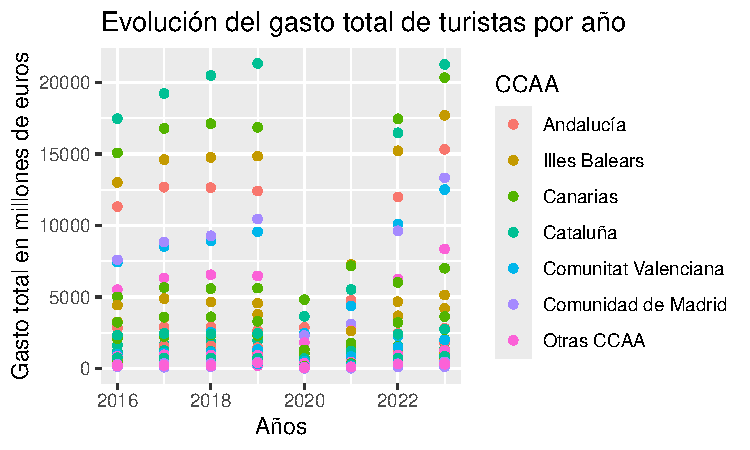
\includegraphics{ProyectoAED2024_Rmd_files/figure-latex/unnamed-chunk-21-1.pdf}

\begin{Shaded}
\begin{Highlighting}[]
\CommentTok{\# Nos centramos en un año en concreto y visualizamos el}
\CommentTok{\# gasto total por país en ese año}
\FunctionTok{ggplot}\NormalTok{(datos[datos}\SpecialCharTok{$}\NormalTok{Periodo }\SpecialCharTok{==} \DecValTok{2023}\NormalTok{, ], }\FunctionTok{aes}\NormalTok{(}\AttributeTok{x =} \FunctionTok{reorder}\NormalTok{(Pais,}
    \SpecialCharTok{{-}}\NormalTok{Gasto\_total), }\AttributeTok{y =}\NormalTok{ Gasto\_total)) }\SpecialCharTok{+} \FunctionTok{geom\_bar}\NormalTok{(}\AttributeTok{stat =} \StringTok{"identity"}\NormalTok{,}
    \FunctionTok{aes}\NormalTok{(}\AttributeTok{fill =}\NormalTok{ Pais)) }\SpecialCharTok{+} \FunctionTok{coord\_flip}\NormalTok{() }\SpecialCharTok{+} \FunctionTok{labs}\NormalTok{(}\AttributeTok{title =} \StringTok{"Gasto por país de residencia en 2023"}\NormalTok{,}
    \AttributeTok{x =} \StringTok{"Gasto total en millones de euros"}\NormalTok{, }\AttributeTok{y =} \StringTok{"País"}\NormalTok{) }\SpecialCharTok{+} \FunctionTok{theme}\NormalTok{(}\AttributeTok{legend.position =} \StringTok{"none"}\NormalTok{)}
\end{Highlighting}
\end{Shaded}

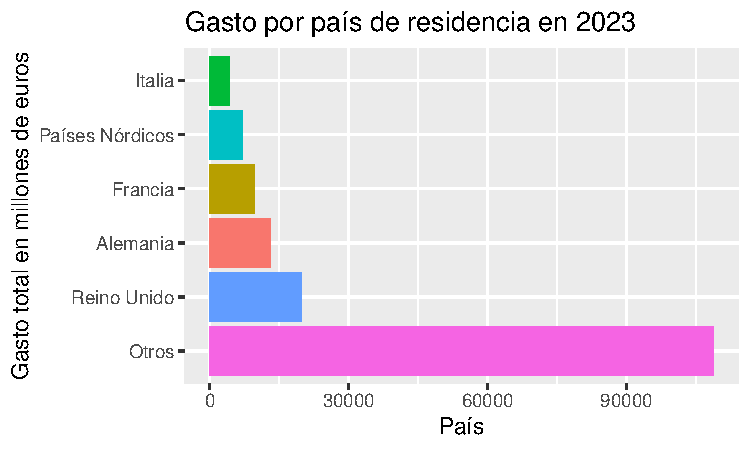
\includegraphics{ProyectoAED2024_Rmd_files/figure-latex/unnamed-chunk-21-2.pdf}

\begin{Shaded}
\begin{Highlighting}[]
\CommentTok{\# Para analizar únicamente una variable por país en una}
\CommentTok{\# sola Comunidad Autónoma.}
\FunctionTok{ggplot}\NormalTok{(datos, }\FunctionTok{aes}\NormalTok{(}\AttributeTok{x =}\NormalTok{ Pais, }\AttributeTok{y =}\NormalTok{ Duracion\_media)) }\SpecialCharTok{+} \FunctionTok{geom\_bar}\NormalTok{(}\AttributeTok{stat =} \StringTok{"identity"}\NormalTok{,}
    \AttributeTok{fill =} \StringTok{"red"}\NormalTok{) }\SpecialCharTok{+} \FunctionTok{facet\_grid}\NormalTok{(. }\SpecialCharTok{\textasciitilde{}}\NormalTok{ CCAA[}\StringTok{"i"}\NormalTok{], }\AttributeTok{scales =} \StringTok{"free"}\NormalTok{) }\SpecialCharTok{+}
    \FunctionTok{labs}\NormalTok{(}\AttributeTok{title =} \StringTok{"Duración media del viaje por país en Andalucía"}\NormalTok{,}
        \AttributeTok{x =} \StringTok{"País"}\NormalTok{, }\AttributeTok{y =} \StringTok{"Duración media del viaje"}\NormalTok{)}
\end{Highlighting}
\end{Shaded}

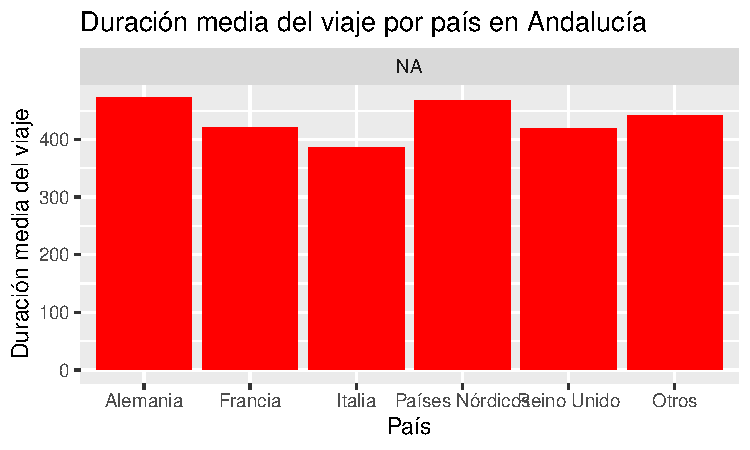
\includegraphics{ProyectoAED2024_Rmd_files/figure-latex/unnamed-chunk-21-3.pdf}

\begin{Shaded}
\begin{Highlighting}[]
\CommentTok{\# Para todas las Comunidades Autónomas por separado}
\FunctionTok{ggplot}\NormalTok{(datos, }\FunctionTok{aes}\NormalTok{(}\AttributeTok{x =}\NormalTok{ Pais, }\AttributeTok{y =}\NormalTok{ Duracion\_media)) }\SpecialCharTok{+} \FunctionTok{geom\_bar}\NormalTok{(}\AttributeTok{stat =} \StringTok{"identity"}\NormalTok{,}
    \AttributeTok{fill =} \StringTok{"purple"}\NormalTok{) }\SpecialCharTok{+} \FunctionTok{facet\_wrap}\NormalTok{(}\SpecialCharTok{\textasciitilde{}}\NormalTok{CCAA, }\AttributeTok{scales =} \StringTok{"free\_y"}\NormalTok{) }\SpecialCharTok{+}
    \FunctionTok{labs}\NormalTok{(}\AttributeTok{title =} \StringTok{"Duración media del viaje por país en cada Comunidad Autónoma"}\NormalTok{,}
        \AttributeTok{x =} \StringTok{"País"}\NormalTok{, }\AttributeTok{y =} \StringTok{"Duración media del viaje"}\NormalTok{) }\SpecialCharTok{+} \FunctionTok{theme}\NormalTok{(}\AttributeTok{axis.text.x =} \FunctionTok{element\_text}\NormalTok{(}\AttributeTok{angle =} \DecValTok{90}\NormalTok{,}
    \AttributeTok{hjust =} \DecValTok{1}\NormalTok{))}
\end{Highlighting}
\end{Shaded}

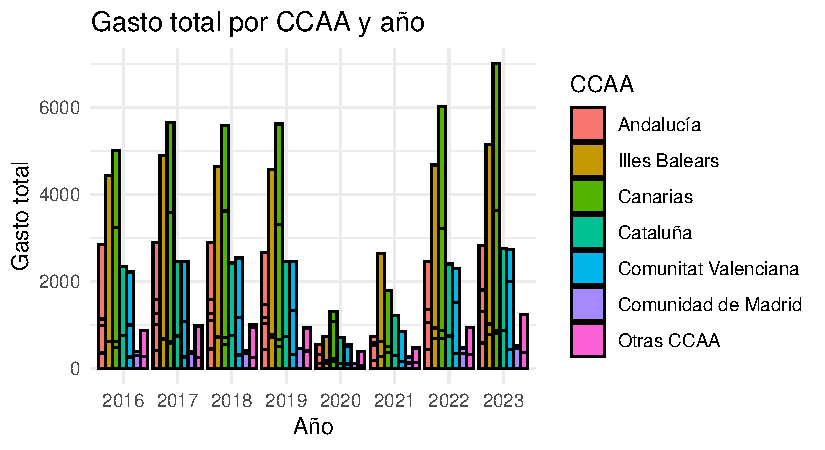
\includegraphics{ProyectoAED2024_Rmd_files/figure-latex/unnamed-chunk-22-1.pdf}

\section{Probamos a analizar el efecto del COVID en el gasto de los
turistas, así como los países que más reducieron su gasto debido a la
pandemia.}\label{probamos-a-analizar-el-efecto-del-covid-en-el-gasto-de-los-turistas-asuxed-como-los-pauxedses-que-muxe1s-reducieron-su-gasto-debido-a-la-pandemia.}

\begin{Shaded}
\begin{Highlighting}[]
\FunctionTok{library}\NormalTok{(tidyr)}

\NormalTok{covid }\OtherTok{\textless{}{-}}\NormalTok{ datos[datos}\SpecialCharTok{$}\NormalTok{Periodo }\SpecialCharTok{==} \DecValTok{2020}\NormalTok{, ]}
\NormalTok{no\_covid }\OtherTok{\textless{}{-}}\NormalTok{ datos[datos}\SpecialCharTok{$}\NormalTok{Periodo }\SpecialCharTok{!=} \DecValTok{2020}\NormalTok{, ]}
\NormalTok{media\_sin\_covid }\OtherTok{\textless{}{-}} \FunctionTok{mean}\NormalTok{(no\_covid}\SpecialCharTok{$}\NormalTok{Gasto\_total[])}
\NormalTok{media\_covid }\OtherTok{\textless{}{-}} \FunctionTok{mean}\NormalTok{(covid}\SpecialCharTok{$}\NormalTok{Gasto\_total)}
\FunctionTok{cat}\NormalTok{(}\StringTok{"La media del gasto total durante el COVID es de"}\NormalTok{, media\_covid,}
    \StringTok{"millones de euros}\SpecialCharTok{\textbackslash{}n}\StringTok{"}\NormalTok{)}
\end{Highlighting}
\end{Shaded}

\begin{verbatim}
## La media del gasto total durante el COVID es de 719.3212 millones de euros
\end{verbatim}

\begin{Shaded}
\begin{Highlighting}[]
\FunctionTok{cat}\NormalTok{(}\StringTok{"Mientras que sin COVID es de"}\NormalTok{, media\_sin\_covid, }\StringTok{"millones de euros}\SpecialCharTok{\textbackslash{}n}\StringTok{"}\NormalTok{)}
\end{Highlighting}
\end{Shaded}

\begin{verbatim}
## Mientras que sin COVID es de 2999.059 millones de euros
\end{verbatim}

\begin{Shaded}
\begin{Highlighting}[]
\NormalTok{datos }\SpecialCharTok{\%\textgreater{}\%}
    \FunctionTok{ggplot}\NormalTok{(}\FunctionTok{aes}\NormalTok{(}\AttributeTok{x =} \FunctionTok{factor}\NormalTok{(Periodo), }\AttributeTok{y =}\NormalTok{ Gasto\_total, }\AttributeTok{fill =}\NormalTok{ (Periodo }\SpecialCharTok{==}
        \DecValTok{2020}\NormalTok{))) }\SpecialCharTok{+} \FunctionTok{geom\_bar}\NormalTok{(}\AttributeTok{stat =} \StringTok{"identity"}\NormalTok{) }\SpecialCharTok{+} \FunctionTok{scale\_fill\_manual}\NormalTok{(}\AttributeTok{values =} \FunctionTok{c}\NormalTok{(}\StringTok{"grey"}\NormalTok{,}
    \StringTok{"red"}\NormalTok{)) }\SpecialCharTok{+} \FunctionTok{labs}\NormalTok{(}\AttributeTok{x =} \StringTok{"Año"}\NormalTok{, }\AttributeTok{y =} \StringTok{"Gasto Total de Turistas"}\NormalTok{,}
    \AttributeTok{title =} \StringTok{"Comparación del Gasto Total de Turistas por Año"}\NormalTok{) }\SpecialCharTok{+}
    \FunctionTok{theme\_minimal}\NormalTok{() }\SpecialCharTok{+} \FunctionTok{theme}\NormalTok{(}\AttributeTok{legend.position =} \StringTok{"none"}\NormalTok{)}
\end{Highlighting}
\end{Shaded}

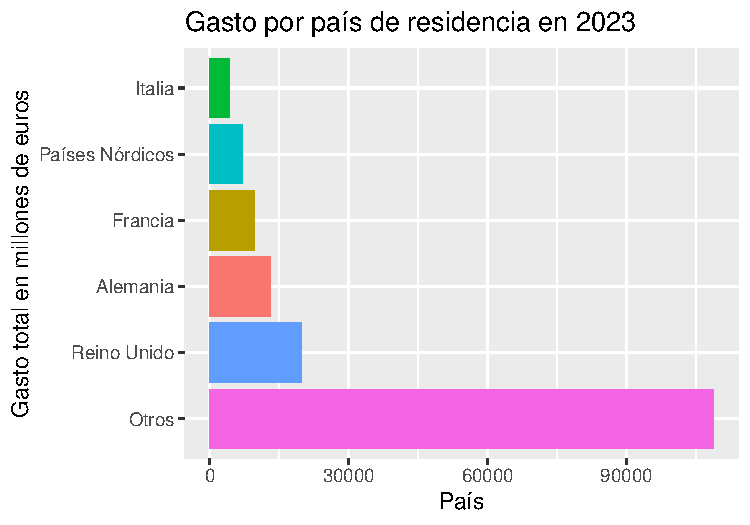
\includegraphics{ProyectoAED2024_Rmd_files/figure-latex/unnamed-chunk-23-1.pdf}

\begin{Shaded}
\begin{Highlighting}[]
\NormalTok{covid\_sin\_otros }\OtherTok{\textless{}{-}}\NormalTok{ covid[covid}\SpecialCharTok{$}\NormalTok{Pais }\SpecialCharTok{!=} \StringTok{"Otros"}\NormalTok{, ]  }\CommentTok{\# Elimino los datos correspondientes a otros países ya que son una suma y no se representa correctamente la tendencia.}
\NormalTok{covid\_sin\_otros }\SpecialCharTok{\%\textgreater{}\%}
    \FunctionTok{ggplot}\NormalTok{(}\FunctionTok{aes}\NormalTok{(}\AttributeTok{x =}\NormalTok{ Pais, }\AttributeTok{y =}\NormalTok{ Gasto\_total, }\AttributeTok{fill =}\NormalTok{ Pais)) }\SpecialCharTok{+} \FunctionTok{geom\_bar}\NormalTok{(}\AttributeTok{stat =} \StringTok{"identity"}\NormalTok{) }\SpecialCharTok{+}
    \FunctionTok{labs}\NormalTok{(}\AttributeTok{title =} \StringTok{"Gasto total de los distintos países durante el COVID"}\NormalTok{)  }\CommentTok{\# Reino Unido gastó más en COVID que el resto de países, Italia el que menos.}
\end{Highlighting}
\end{Shaded}

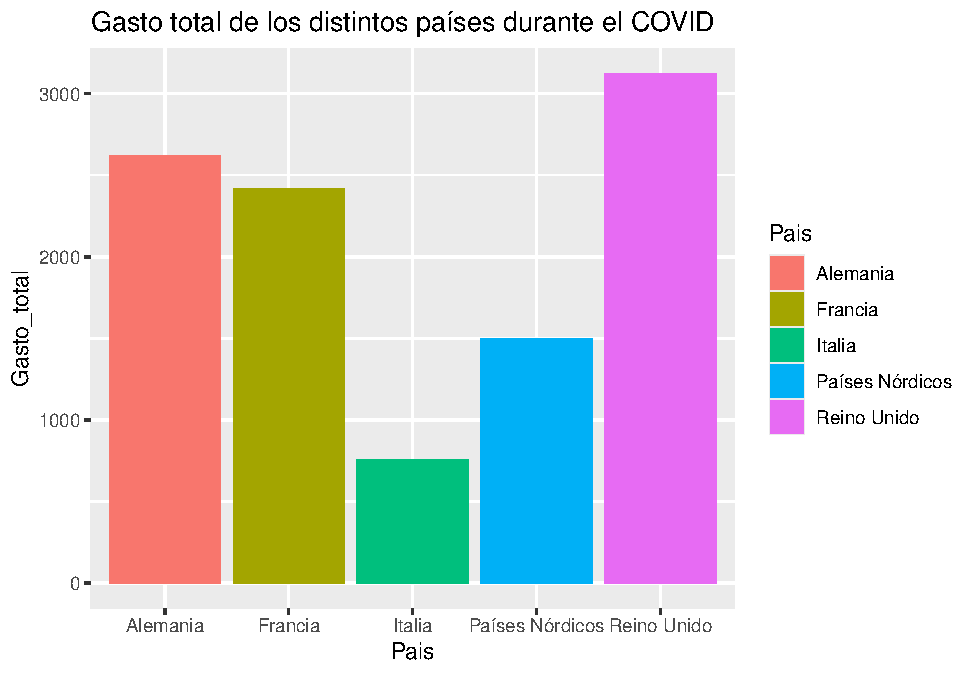
\includegraphics{ProyectoAED2024_Rmd_files/figure-latex/unnamed-chunk-23-2.pdf}

\begin{Shaded}
\begin{Highlighting}[]
\CommentTok{\# ¿En qué comunidad autónoma se viajó más durante el COVID?}
\NormalTok{covid\_sin\_otros }\SpecialCharTok{\%\textgreater{}\%}
    \FunctionTok{ggplot}\NormalTok{(}\FunctionTok{aes}\NormalTok{(}\AttributeTok{x =}\NormalTok{ CCAA, }\AttributeTok{y =}\NormalTok{ Gasto\_total, }\AttributeTok{fill =}\NormalTok{ CCAA)) }\SpecialCharTok{+} \FunctionTok{geom\_bar}\NormalTok{(}\AttributeTok{stat =} \StringTok{"identity"}\NormalTok{) }\SpecialCharTok{+}
    \FunctionTok{labs}\NormalTok{(}\AttributeTok{title =} \StringTok{"Gasto total en las distintas comunidades autónomas durante el COVID"}\NormalTok{)}
\end{Highlighting}
\end{Shaded}

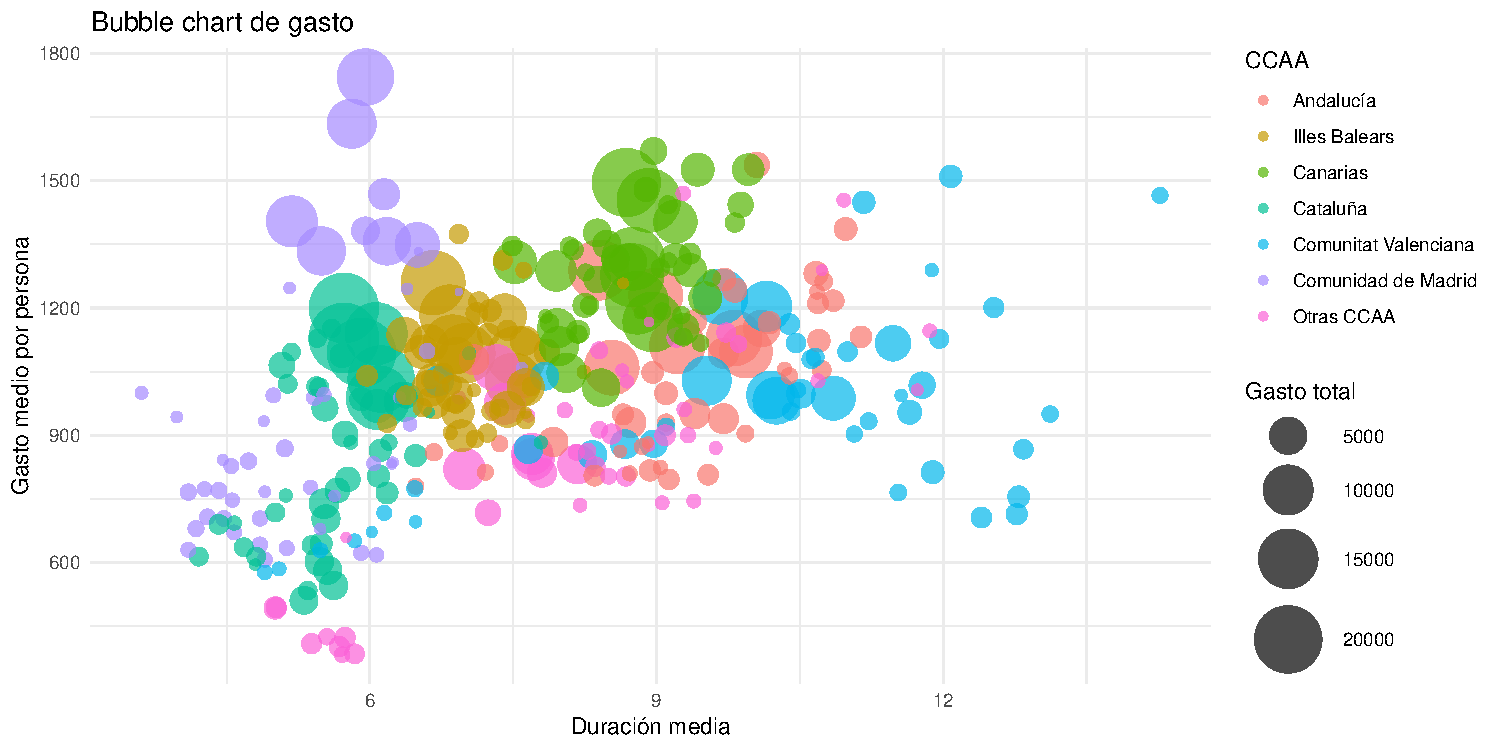
\includegraphics{ProyectoAED2024_Rmd_files/figure-latex/unnamed-chunk-24-1.pdf}

\begin{Shaded}
\begin{Highlighting}[]
\CommentTok{\# En Canarias el gasto de turistas fue mayor que en el}
\CommentTok{\# resto de Comunidades Autónomas durante el COVID, ¿menor}
\CommentTok{\# regulación?}
\end{Highlighting}
\end{Shaded}

Filtraremos los datos totales por el Periodo y recogeremos solo la
variable que nos sirve para representar la magnitud de valores en el
mapa de visualización, en este caso el gasto medio por persona

\begin{Shaded}
\begin{Highlighting}[]
\CommentTok{\# Tomamos los distintos periodos que existen en nuestro}
\CommentTok{\# conjunto de datos para diferenciar temporalmente}
\NormalTok{periodos }\OtherTok{\textless{}{-}} \FunctionTok{unique}\NormalTok{(datos\_total\_por\_residencia}\SpecialCharTok{$}\NormalTok{Periodo)}

\CommentTok{\# Separamos los gastos por países Nórdicos y el resto ya}
\CommentTok{\# que se querrá hacer una subdivisión más para estos}
\NormalTok{datos\_total\_residencia }\OtherTok{\textless{}{-}}\NormalTok{ datos\_total\_por\_residencia }\SpecialCharTok{\%\textgreater{}\%}
    \FunctionTok{select}\NormalTok{(Pais, Gasto\_total, Gasto\_medio\_persona, Gasto\_medio\_diario\_persona,}
\NormalTok{        Duracion\_media, Periodo) }\SpecialCharTok{\%\textgreater{}\%}
    \FunctionTok{filter}\NormalTok{(Periodo }\SpecialCharTok{\%in\%}\NormalTok{ periodos }\SpecialCharTok{\&}\NormalTok{ Pais }\SpecialCharTok{!=} \StringTok{"Total"}\NormalTok{)}

\NormalTok{datos\_total\_residencia\_PN }\OtherTok{\textless{}{-}}\NormalTok{ datos\_total\_residencia }\SpecialCharTok{\%\textgreater{}\%}
    \FunctionTok{select}\NormalTok{(Pais, Gasto\_total, Gasto\_medio\_persona, Gasto\_medio\_diario\_persona,}
\NormalTok{        Duracion\_media, Periodo) }\SpecialCharTok{\%\textgreater{}\%}
    \FunctionTok{filter}\NormalTok{(Pais }\SpecialCharTok{==} \StringTok{"Países Nórdicos"}\NormalTok{)}

\CommentTok{\# Introducimos 4 filas iguales sobre los países nórdicos}
\CommentTok{\# para separar con el join estos y poder representarlos en}
\CommentTok{\# el mapa}

\NormalTok{datos\_total\_residencia }\OtherTok{\textless{}{-}} \FunctionTok{rbind}\NormalTok{(datos\_total\_residencia, datos\_total\_residencia\_PN,}
\NormalTok{    datos\_total\_residencia\_PN, datos\_total\_residencia\_PN, datos\_total\_residencia\_PN)}

\CommentTok{\# El ano de referencia de los mapas determina el año en que}
\CommentTok{\# se recogió la información de las coordenadas y la}
\CommentTok{\# división de los países (como no hay ninguna división o}
\CommentTok{\# cambio de coordenadas importante para los países y los}
\CommentTok{\# períodos importantes no es muy relevante)}
\NormalTok{año\_ref }\OtherTok{\textless{}{-}} \DecValTok{2020}

\CommentTok{\# Datos}
\NormalTok{countries }\OtherTok{\textless{}{-}} \FunctionTok{gisco\_get\_countries}\NormalTok{(}\AttributeTok{year =}\NormalTok{ año\_ref, }\AttributeTok{resolution =} \DecValTok{20}\NormalTok{) }\SpecialCharTok{\%\textgreater{}\%}
    \FunctionTok{select}\NormalTok{(CNTR\_ID, NAME\_ENGL, geometry) }\SpecialCharTok{\%\textgreater{}\%}
    \FunctionTok{st\_transform}\NormalTok{(}\DecValTok{3035}\NormalTok{)}

\CommentTok{\# En los datos que podemos recoger de la librería que nos}
\CommentTok{\# determina las coordenadas de los países necesitamos}
\CommentTok{\# filtrar por los que vamos a estudiar en base a nuestro}
\CommentTok{\# conjunto de datos.}
\NormalTok{paises\_english }\OtherTok{\textless{}{-}} \FunctionTok{c}\NormalTok{(}\StringTok{"United Kingdom"}\NormalTok{, }\StringTok{"Denmark"}\NormalTok{, }\StringTok{"Germany"}\NormalTok{, }\StringTok{"France"}\NormalTok{,}
    \StringTok{"Italy"}\NormalTok{, }\StringTok{"Sweden"}\NormalTok{, }\StringTok{"Norway"}\NormalTok{, }\StringTok{"Iceland"}\NormalTok{, }\StringTok{"Finland"}\NormalTok{)}
\NormalTok{countries\_filtered }\OtherTok{\textless{}{-}}\NormalTok{ countries }\SpecialCharTok{\%\textgreater{}\%}
    \FunctionTok{filter}\NormalTok{(NAME\_ENGL }\SpecialCharTok{\%in\%}\NormalTok{ paises\_english)}

\CommentTok{\# Incluir columna de identificación de los países para unir}
\CommentTok{\# con las coordenadas de los mapas}
\NormalTok{CNTR\_ID }\OtherTok{\textless{}{-}} \FunctionTok{c}\NormalTok{(}\StringTok{"UK"}\NormalTok{, }\StringTok{"DK"}\NormalTok{, }\StringTok{"DE"}\NormalTok{, }\StringTok{"FR"}\NormalTok{, }\StringTok{"IT"}\NormalTok{, }\StringTok{"SE"}\NormalTok{, }\StringTok{"NO"}\NormalTok{, }\StringTok{"IS"}\NormalTok{,}
    \StringTok{"FI"}\NormalTok{)}
\NormalTok{Country\_Ids }\OtherTok{\textless{}{-}} \FunctionTok{c}\NormalTok{()}
\ControlFlowTok{for}\NormalTok{ (pais }\ControlFlowTok{in}\NormalTok{ CNTR\_ID) \{}
\NormalTok{    Country\_aux }\OtherTok{\textless{}{-}} \FunctionTok{rep}\NormalTok{(pais, }\AttributeTok{times =} \FunctionTok{length}\NormalTok{(periodos))}
\NormalTok{    Country\_Ids }\OtherTok{\textless{}{-}} \FunctionTok{c}\NormalTok{(Country\_Ids, Country\_aux)}
\NormalTok{\}}

\NormalTok{datos\_total\_residencia }\OtherTok{\textless{}{-}} \FunctionTok{cbind}\NormalTok{(datos\_total\_residencia, Country\_Ids)}


\NormalTok{datos\_total\_residencia\_viz }\OtherTok{\textless{}{-}}\NormalTok{ datos\_total\_residencia }\SpecialCharTok{\%\textgreater{}\%}
    \FunctionTok{left\_join}\NormalTok{(countries, }\AttributeTok{by =} \FunctionTok{join\_by}\NormalTok{(Country\_Ids }\SpecialCharTok{==}\NormalTok{ CNTR\_ID))}



\CommentTok{\# Mapa base}
\NormalTok{geographic\_map\_gasto\_medio }\OtherTok{\textless{}{-}} \FunctionTok{ggplot}\NormalTok{(datos\_total\_residencia\_viz) }\SpecialCharTok{+}
    \FunctionTok{geom\_sf}\NormalTok{(}\FunctionTok{aes}\NormalTok{(}\AttributeTok{geometry =}\NormalTok{ geometry, }\AttributeTok{fill =}\NormalTok{ Gasto\_medio\_persona),}
        \AttributeTok{linewidth =} \FloatTok{0.5}\NormalTok{) }\SpecialCharTok{+} \FunctionTok{facet\_wrap}\NormalTok{(}\SpecialCharTok{\textasciitilde{}}\NormalTok{Periodo) }\SpecialCharTok{+} \FunctionTok{theme}\NormalTok{(}\AttributeTok{axis.text.x =} \FunctionTok{element\_blank}\NormalTok{(),}
    \AttributeTok{axis.text.y =} \FunctionTok{element\_blank}\NormalTok{(), }\AttributeTok{axis.ticks =} \FunctionTok{element\_blank}\NormalTok{())}

\NormalTok{geographic\_map\_gasto\_medio }\OtherTok{\textless{}{-}}\NormalTok{ geographic\_map\_gasto\_medio }\SpecialCharTok{+} \FunctionTok{xlim}\NormalTok{(}\FunctionTok{c}\NormalTok{(}\DecValTok{2200000}\NormalTok{,}
    \DecValTok{7150000}\NormalTok{)) }\SpecialCharTok{+} \FunctionTok{ylim}\NormalTok{(}\FunctionTok{c}\NormalTok{(}\DecValTok{1380000}\NormalTok{, }\DecValTok{5500000}\NormalTok{)) }\SpecialCharTok{+} \FunctionTok{geom\_sf\_interactive}\NormalTok{(}\AttributeTok{fill =} \ConstantTok{NA}\NormalTok{,}
    \FunctionTok{aes}\NormalTok{(}\AttributeTok{data\_id =}\NormalTok{ Country\_Ids, }\AttributeTok{geometry =}\NormalTok{ geometry, }\AttributeTok{tooltip =}\NormalTok{ Gasto\_medio\_persona),}
    \AttributeTok{color =} \StringTok{"black"}\NormalTok{, }\AttributeTok{linewidth =} \FloatTok{0.1}\NormalTok{)}
\FunctionTok{girafe}\NormalTok{(}\AttributeTok{ggobj =}\NormalTok{ geographic\_map\_gasto\_medio)}
\end{Highlighting}
\end{Shaded}

\begin{Shaded}
\begin{Highlighting}[]
\CommentTok{\# Marta: Te comenté esta parte porque me estaba dando}
\CommentTok{\# problemas al hacer knit no se por qué}

\CommentTok{\# Gráfico ggplot(datos\_total\_residencia\_viz) + \# Primera}
\CommentTok{\# capa con todos los países geom\_sf(aes(geometry=}
\CommentTok{\# geometry), data = datos\_total\_residencia\_viz, fill =}
\CommentTok{\# \textquotesingle{}grey80\textquotesingle{}, color = NA) + \# Establece límites}
\CommentTok{\# xlim(c(2200000, 7150000)) + ylim(c(1380000, 5500000))}
\end{Highlighting}
\end{Shaded}

\begin{Shaded}
\begin{Highlighting}[]
\NormalTok{geographic\_map\_gasto\_medio\_diario }\OtherTok{\textless{}{-}} \FunctionTok{ggplot}\NormalTok{(datos\_total\_residencia\_viz) }\SpecialCharTok{+}
    \FunctionTok{geom\_sf}\NormalTok{(}\FunctionTok{aes}\NormalTok{(}\AttributeTok{geometry =}\NormalTok{ geometry, }\AttributeTok{fill =}\NormalTok{ Gasto\_medio\_diario\_persona),}
        \AttributeTok{linewidth =} \FloatTok{0.5}\NormalTok{) }\SpecialCharTok{+} \FunctionTok{facet\_wrap}\NormalTok{(}\SpecialCharTok{\textasciitilde{}}\NormalTok{Periodo) }\SpecialCharTok{+} \FunctionTok{theme}\NormalTok{(}\AttributeTok{axis.text.x =} \FunctionTok{element\_blank}\NormalTok{(),}
    \AttributeTok{axis.text.y =} \FunctionTok{element\_blank}\NormalTok{(), }\AttributeTok{axis.ticks =} \FunctionTok{element\_blank}\NormalTok{())}

\NormalTok{geographic\_map\_gasto\_medio\_diario }\OtherTok{\textless{}{-}}\NormalTok{ geographic\_map\_gasto\_medio\_diario }\SpecialCharTok{+}
    \FunctionTok{xlim}\NormalTok{(}\FunctionTok{c}\NormalTok{(}\DecValTok{2200000}\NormalTok{, }\DecValTok{7150000}\NormalTok{)) }\SpecialCharTok{+} \FunctionTok{ylim}\NormalTok{(}\FunctionTok{c}\NormalTok{(}\DecValTok{1380000}\NormalTok{, }\DecValTok{5500000}\NormalTok{)) }\SpecialCharTok{+} \FunctionTok{geom\_sf\_interactive}\NormalTok{(}\AttributeTok{fill =} \ConstantTok{NA}\NormalTok{,}
    \FunctionTok{aes}\NormalTok{(}\AttributeTok{data\_id =}\NormalTok{ Country\_Ids, }\AttributeTok{geometry =}\NormalTok{ geometry, }\AttributeTok{tooltip =}\NormalTok{ Gasto\_medio\_diario\_persona),}
    \AttributeTok{color =} \StringTok{"black"}\NormalTok{, }\AttributeTok{linewidth =} \FloatTok{0.1}\NormalTok{)}
\FunctionTok{girafe}\NormalTok{(}\AttributeTok{ggobj =}\NormalTok{ geographic\_map\_gasto\_medio\_diario)}
\end{Highlighting}
\end{Shaded}

\begin{Shaded}
\begin{Highlighting}[]
\NormalTok{geographic\_map\_gasto\_total }\OtherTok{\textless{}{-}} \FunctionTok{ggplot}\NormalTok{(datos\_total\_residencia\_viz) }\SpecialCharTok{+}
    \FunctionTok{geom\_sf}\NormalTok{(}\FunctionTok{aes}\NormalTok{(}\AttributeTok{geometry =}\NormalTok{ geometry, }\AttributeTok{fill =}\NormalTok{ Gasto\_total), }\AttributeTok{linewidth =} \FloatTok{0.5}\NormalTok{) }\SpecialCharTok{+}
    \FunctionTok{facet\_wrap}\NormalTok{(}\SpecialCharTok{\textasciitilde{}}\NormalTok{Periodo) }\SpecialCharTok{+} \FunctionTok{theme}\NormalTok{(}\AttributeTok{axis.text.x =} \FunctionTok{element\_blank}\NormalTok{(),}
    \AttributeTok{axis.text.y =} \FunctionTok{element\_blank}\NormalTok{(), }\AttributeTok{axis.ticks =} \FunctionTok{element\_blank}\NormalTok{())}

\NormalTok{geographic\_map\_gasto\_total }\OtherTok{\textless{}{-}}\NormalTok{ geographic\_map\_gasto\_total }\SpecialCharTok{+} \FunctionTok{xlim}\NormalTok{(}\FunctionTok{c}\NormalTok{(}\DecValTok{2200000}\NormalTok{,}
    \DecValTok{7150000}\NormalTok{)) }\SpecialCharTok{+} \FunctionTok{ylim}\NormalTok{(}\FunctionTok{c}\NormalTok{(}\DecValTok{1380000}\NormalTok{, }\DecValTok{5500000}\NormalTok{)) }\SpecialCharTok{+} \FunctionTok{geom\_sf\_interactive}\NormalTok{(}\AttributeTok{fill =} \ConstantTok{NA}\NormalTok{,}
    \FunctionTok{aes}\NormalTok{(}\AttributeTok{data\_id =}\NormalTok{ Country\_Ids, }\AttributeTok{geometry =}\NormalTok{ geometry, }\AttributeTok{tooltip =}\NormalTok{ Gasto\_total),}
    \AttributeTok{color =} \StringTok{"black"}\NormalTok{, }\AttributeTok{linewidth =} \FloatTok{0.1}\NormalTok{)}
\FunctionTok{girafe}\NormalTok{(}\AttributeTok{ggobj =}\NormalTok{ geographic\_map\_gasto\_total)}
\end{Highlighting}
\end{Shaded}

\begin{Shaded}
\begin{Highlighting}[]
\NormalTok{geographic\_map\_duracion\_media }\OtherTok{\textless{}{-}} \FunctionTok{ggplot}\NormalTok{(datos\_total\_residencia\_viz) }\SpecialCharTok{+}
    \FunctionTok{geom\_sf}\NormalTok{(}\FunctionTok{aes}\NormalTok{(}\AttributeTok{geometry =}\NormalTok{ geometry, }\AttributeTok{fill =}\NormalTok{ Duracion\_media),}
        \AttributeTok{linewidth =} \FloatTok{0.5}\NormalTok{) }\SpecialCharTok{+} \FunctionTok{facet\_wrap}\NormalTok{(}\SpecialCharTok{\textasciitilde{}}\NormalTok{Periodo) }\SpecialCharTok{+} \FunctionTok{theme}\NormalTok{(}\AttributeTok{axis.text.x =} \FunctionTok{element\_blank}\NormalTok{(),}
    \AttributeTok{axis.text.y =} \FunctionTok{element\_blank}\NormalTok{(), }\AttributeTok{axis.ticks =} \FunctionTok{element\_blank}\NormalTok{())}

\NormalTok{geographic\_map\_duracion\_media }\OtherTok{\textless{}{-}}\NormalTok{ geographic\_map\_duracion\_media }\SpecialCharTok{+}
    \FunctionTok{xlim}\NormalTok{(}\FunctionTok{c}\NormalTok{(}\DecValTok{2200000}\NormalTok{, }\DecValTok{7150000}\NormalTok{)) }\SpecialCharTok{+} \FunctionTok{ylim}\NormalTok{(}\FunctionTok{c}\NormalTok{(}\DecValTok{1380000}\NormalTok{, }\DecValTok{5500000}\NormalTok{)) }\SpecialCharTok{+} \FunctionTok{geom\_sf\_interactive}\NormalTok{(}\AttributeTok{fill =} \ConstantTok{NA}\NormalTok{,}
    \FunctionTok{aes}\NormalTok{(}\AttributeTok{data\_id =}\NormalTok{ Country\_Ids, }\AttributeTok{geometry =}\NormalTok{ geometry, }\AttributeTok{tooltip =}\NormalTok{ Duracion\_media),}
    \AttributeTok{color =} \StringTok{"black"}\NormalTok{, }\AttributeTok{linewidth =} \FloatTok{0.1}\NormalTok{)}
\FunctionTok{girafe}\NormalTok{(}\AttributeTok{ggobj =}\NormalTok{ geographic\_map\_duracion\_media)}
\end{Highlighting}
\end{Shaded}

\begin{Shaded}
\begin{Highlighting}[]
\CommentTok{\# Datos}
\NormalTok{año\_ref }\OtherTok{\textless{}{-}} \DecValTok{2021}
\NormalTok{spain\_CCAAs }\OtherTok{\textless{}{-}} \FunctionTok{gisco\_get\_nuts}\NormalTok{(}\AttributeTok{year =}\NormalTok{ año\_ref, }\AttributeTok{country =} \StringTok{"Spain"}\NormalTok{,}
    \AttributeTok{resolution =} \DecValTok{20}\NormalTok{)}

\FunctionTok{ggplot}\NormalTok{(spain\_CCAAs) }\SpecialCharTok{+} \FunctionTok{geom\_sf}\NormalTok{(}\FunctionTok{aes}\NormalTok{(}\AttributeTok{geometry =}\NormalTok{ geometry))}
\end{Highlighting}
\end{Shaded}

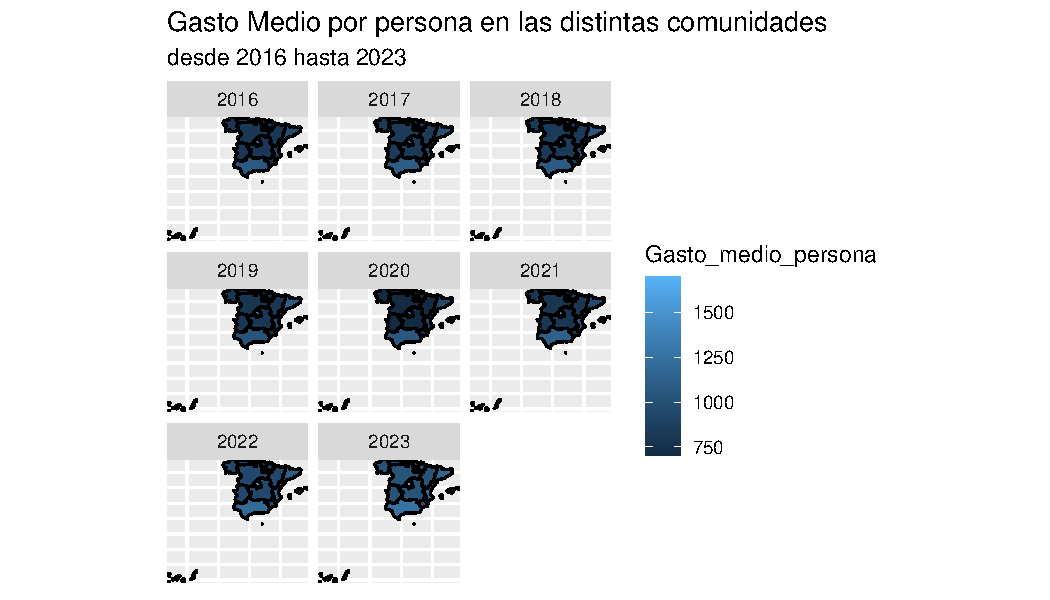
\includegraphics{ProyectoAED2024_Rmd_files/figure-latex/unnamed-chunk-29-1.pdf}

\begin{Shaded}
\begin{Highlighting}[]
\NormalTok{spain\_Comunities }\OtherTok{\textless{}{-}}\NormalTok{ spain\_CCAAs }\SpecialCharTok{\%\textgreater{}\%}
    \FunctionTok{filter}\NormalTok{(LEVL\_CODE }\SpecialCharTok{==} \DecValTok{2}\NormalTok{)}
\NormalTok{spain\_CCAAs }\SpecialCharTok{\%\textgreater{}\%}
    \FunctionTok{ggplot}\NormalTok{(}\FunctionTok{aes}\NormalTok{(}\AttributeTok{geometry =}\NormalTok{ geometry)) }\SpecialCharTok{+} \FunctionTok{geom\_sf}\NormalTok{(}\AttributeTok{data =}\NormalTok{ spain\_Comunities,}
    \FunctionTok{aes}\NormalTok{(}\AttributeTok{fill =}\NormalTok{ NUTS\_NAME), }\AttributeTok{color =} \StringTok{"black"}\NormalTok{, }\AttributeTok{linewidth =} \FloatTok{0.5}\NormalTok{) }\SpecialCharTok{+}
    \FunctionTok{geom\_sf}\NormalTok{(}\AttributeTok{fill =} \ConstantTok{NA}\NormalTok{, }\AttributeTok{color =} \StringTok{"black"}\NormalTok{, }\AttributeTok{linewidth =} \FloatTok{0.1}\NormalTok{)}
\end{Highlighting}
\end{Shaded}

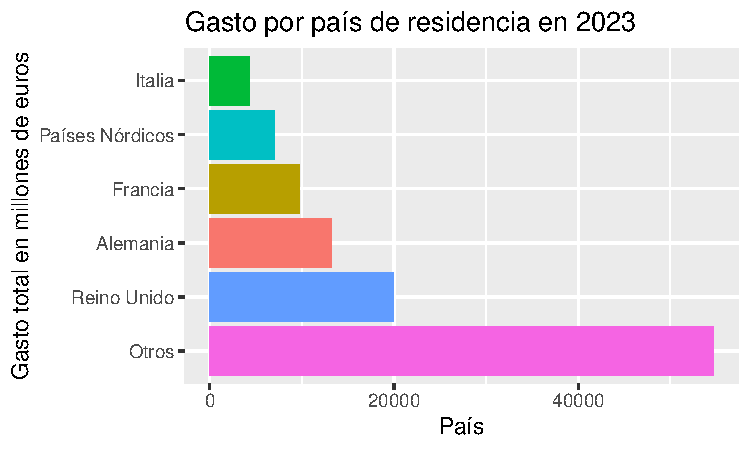
\includegraphics{ProyectoAED2024_Rmd_files/figure-latex/unnamed-chunk-29-2.pdf}

%%%%%%%%%%%%%%%%%%%%%%%%%%%%%%%%%%%%%%%%%%

\vspace{6pt}

%%%%%%%%%%%%%%%%%%%%%%%%%%%%%%%%%%%%%%%%%%
%% optional

% Only for the journal Methods and Protocols:
% If you wish to submit a video article, please do so with any other supplementary material.
% \supplementary{The following supporting information can be downloaded at: \linksupplementary{s1}, Figure S1: title; Table S1: title; Video S1: title. A supporting video article is available at doi: link.}

%%%%%%%%%%%%%%%%%%%%%%%%%%%%%%%%%%%%%%%%%%







%%%%%%%%%%%%%%%%%%%%%%%%%%%%%%%%%%%%%%%%%%
%% Optional

%% Only for journal Encyclopedia


%%%%%%%%%%%%%%%%%%%%%%%%%%%%%%%%%%%%%%%%%%
%% Optional
\input{"appendix.tex"}
%%%%%%%%%%%%%%%%%%%%%%%%%%%%%%%%%%%%%%%%%%
\begin{adjustwidth}{-\extralength}{0cm}

%\printendnotes[custom] % Un-comment to print a list of endnotes


\reftitle{References}
\bibliography{mybibfile.bib}

% If authors have biography, please use the format below
%\section*{Short Biography of Authors}
%\bio
%{\raisebox{-0.35cm}{\includegraphics[width=3.5cm,height=5.3cm,clip,keepaspectratio]{Definitions/author1.pdf}}}
%{\textbf{Firstname Lastname} Biography of first author}
%
%\bio
%{\raisebox{-0.35cm}{\includegraphics[width=3.5cm,height=5.3cm,clip,keepaspectratio]{Definitions/author2.jpg}}}
%{\textbf{Firstname Lastname} Biography of second author}

%%%%%%%%%%%%%%%%%%%%%%%%%%%%%%%%%%%%%%%%%%
%% for journal Sci
%\reviewreports{\\
%Reviewer 1 comments and authors’ response\\
%Reviewer 2 comments and authors’ response\\
%Reviewer 3 comments and authors’ response
%}
%%%%%%%%%%%%%%%%%%%%%%%%%%%%%%%%%%%%%%%%%%
\PublishersNote{}
\end{adjustwidth}


\end{document}
